% !TEX root=/home/tavant/these/manuscript/src/manuscript.tex
\let\oldtheHchapter\theHchapter
\let\oldthechapter\thechapter
\let\oldthechaptername\chaptername

\renewcommand\theHchapter{}
\renewcommand\thechapter{}
\renewcommand\chaptername{}


\newcommand\chaptertitle{ Concepts and preliminaries }

\chapter*{\chaptertitle}
\label{ch-concepts}
% \addcontentsline{toc}{chapter}{Concepts and preliminaries}
\addstarredchapter{\chaptertitle}
 \markboth{\chaptertitle}{}
% \renewcommand\leftmark{\expandafter\MakeUppercase{\chaptertitle}}
% \renewcommand\rightmark{\expandafter\MakeUppercase{\chaptertitle}}
% \epigraph{The Earth is the cradle of humanity, but mankind cannot stay in the cradle forever.}{Konstantin Tsiolkovsky}
% 
% 
% \begin{chapquote}{Konstantin Tsiolkovsky, \textit{pioneer of the astronautic theory}}
% The Earth is the cradle of humanity, but mankind cannot stay in the cradle forever.
% \end{chapquote}


\quotechapt{Konstantin Tsiolkovsky, \textit{pioneer of the astronautic theory}}{
  The Earth is the cradle of humanity, but mankind cannot stay in the cradle forever.\\}


  \minitoc


% !TEX root=/home/tavant/these/manuscript/src/manuscript.tex



\section{Propulsion system for spacecrafts}
\label{sec-propulsion}
% \addcontentsline{toc}{section}{Propulsion system for spacecrafts}


In order to move in space, satellites, scientific probes, and spacecrafts in general rely on a propulsion system.
The cost to go from one location to another can be expressed as $\Delta V$, a measure of impulse needed to maneuver.
\nomenclature[Q]{$\Delta V$}{Measure of impulse needed for a space manoeuvre}
\Cref{fig-subway_DV} illustrates the $\Delta V$ required to evolve in the solar system.
We can see that reaching \ac{LEO} needs a $\Delta V$ of 9400 m/s while the \ac{GEO} is 3910 m/s further.
Landing on the Moon from the Earth ground requires a total of 15 km/s, while landing on Neptune requires $\Delta V =43.7$\,km/s.
For a spacecraft of instantaneous mass $M(t)$, with a propulsion system generating a thrust $T(t)$, the $\Delta V$ between $t_1$ and $t_2$ is
\begin{equation} \label{eq-dv}
  \Delta V = \int_{t_1}^{t_2} \frac{ \norm{T(t)}}{M(t)} dt.
\end{equation}
As expected, we see from \cref{eq-dv} that for a more massive spacecraft, a more intense, or a longer thrust is needed in order to obtain the same $\Delta V$.
\nomenclature[Q]{\ensuremath{ t}}{Time}
\nomenclature[Q]{\ensuremath{ T}}{Thrust}
\nomenclature[Q]{\ensuremath{ M}}{Mass of a spacecraft}
\begin{figure}[!hbt]
  \centering
  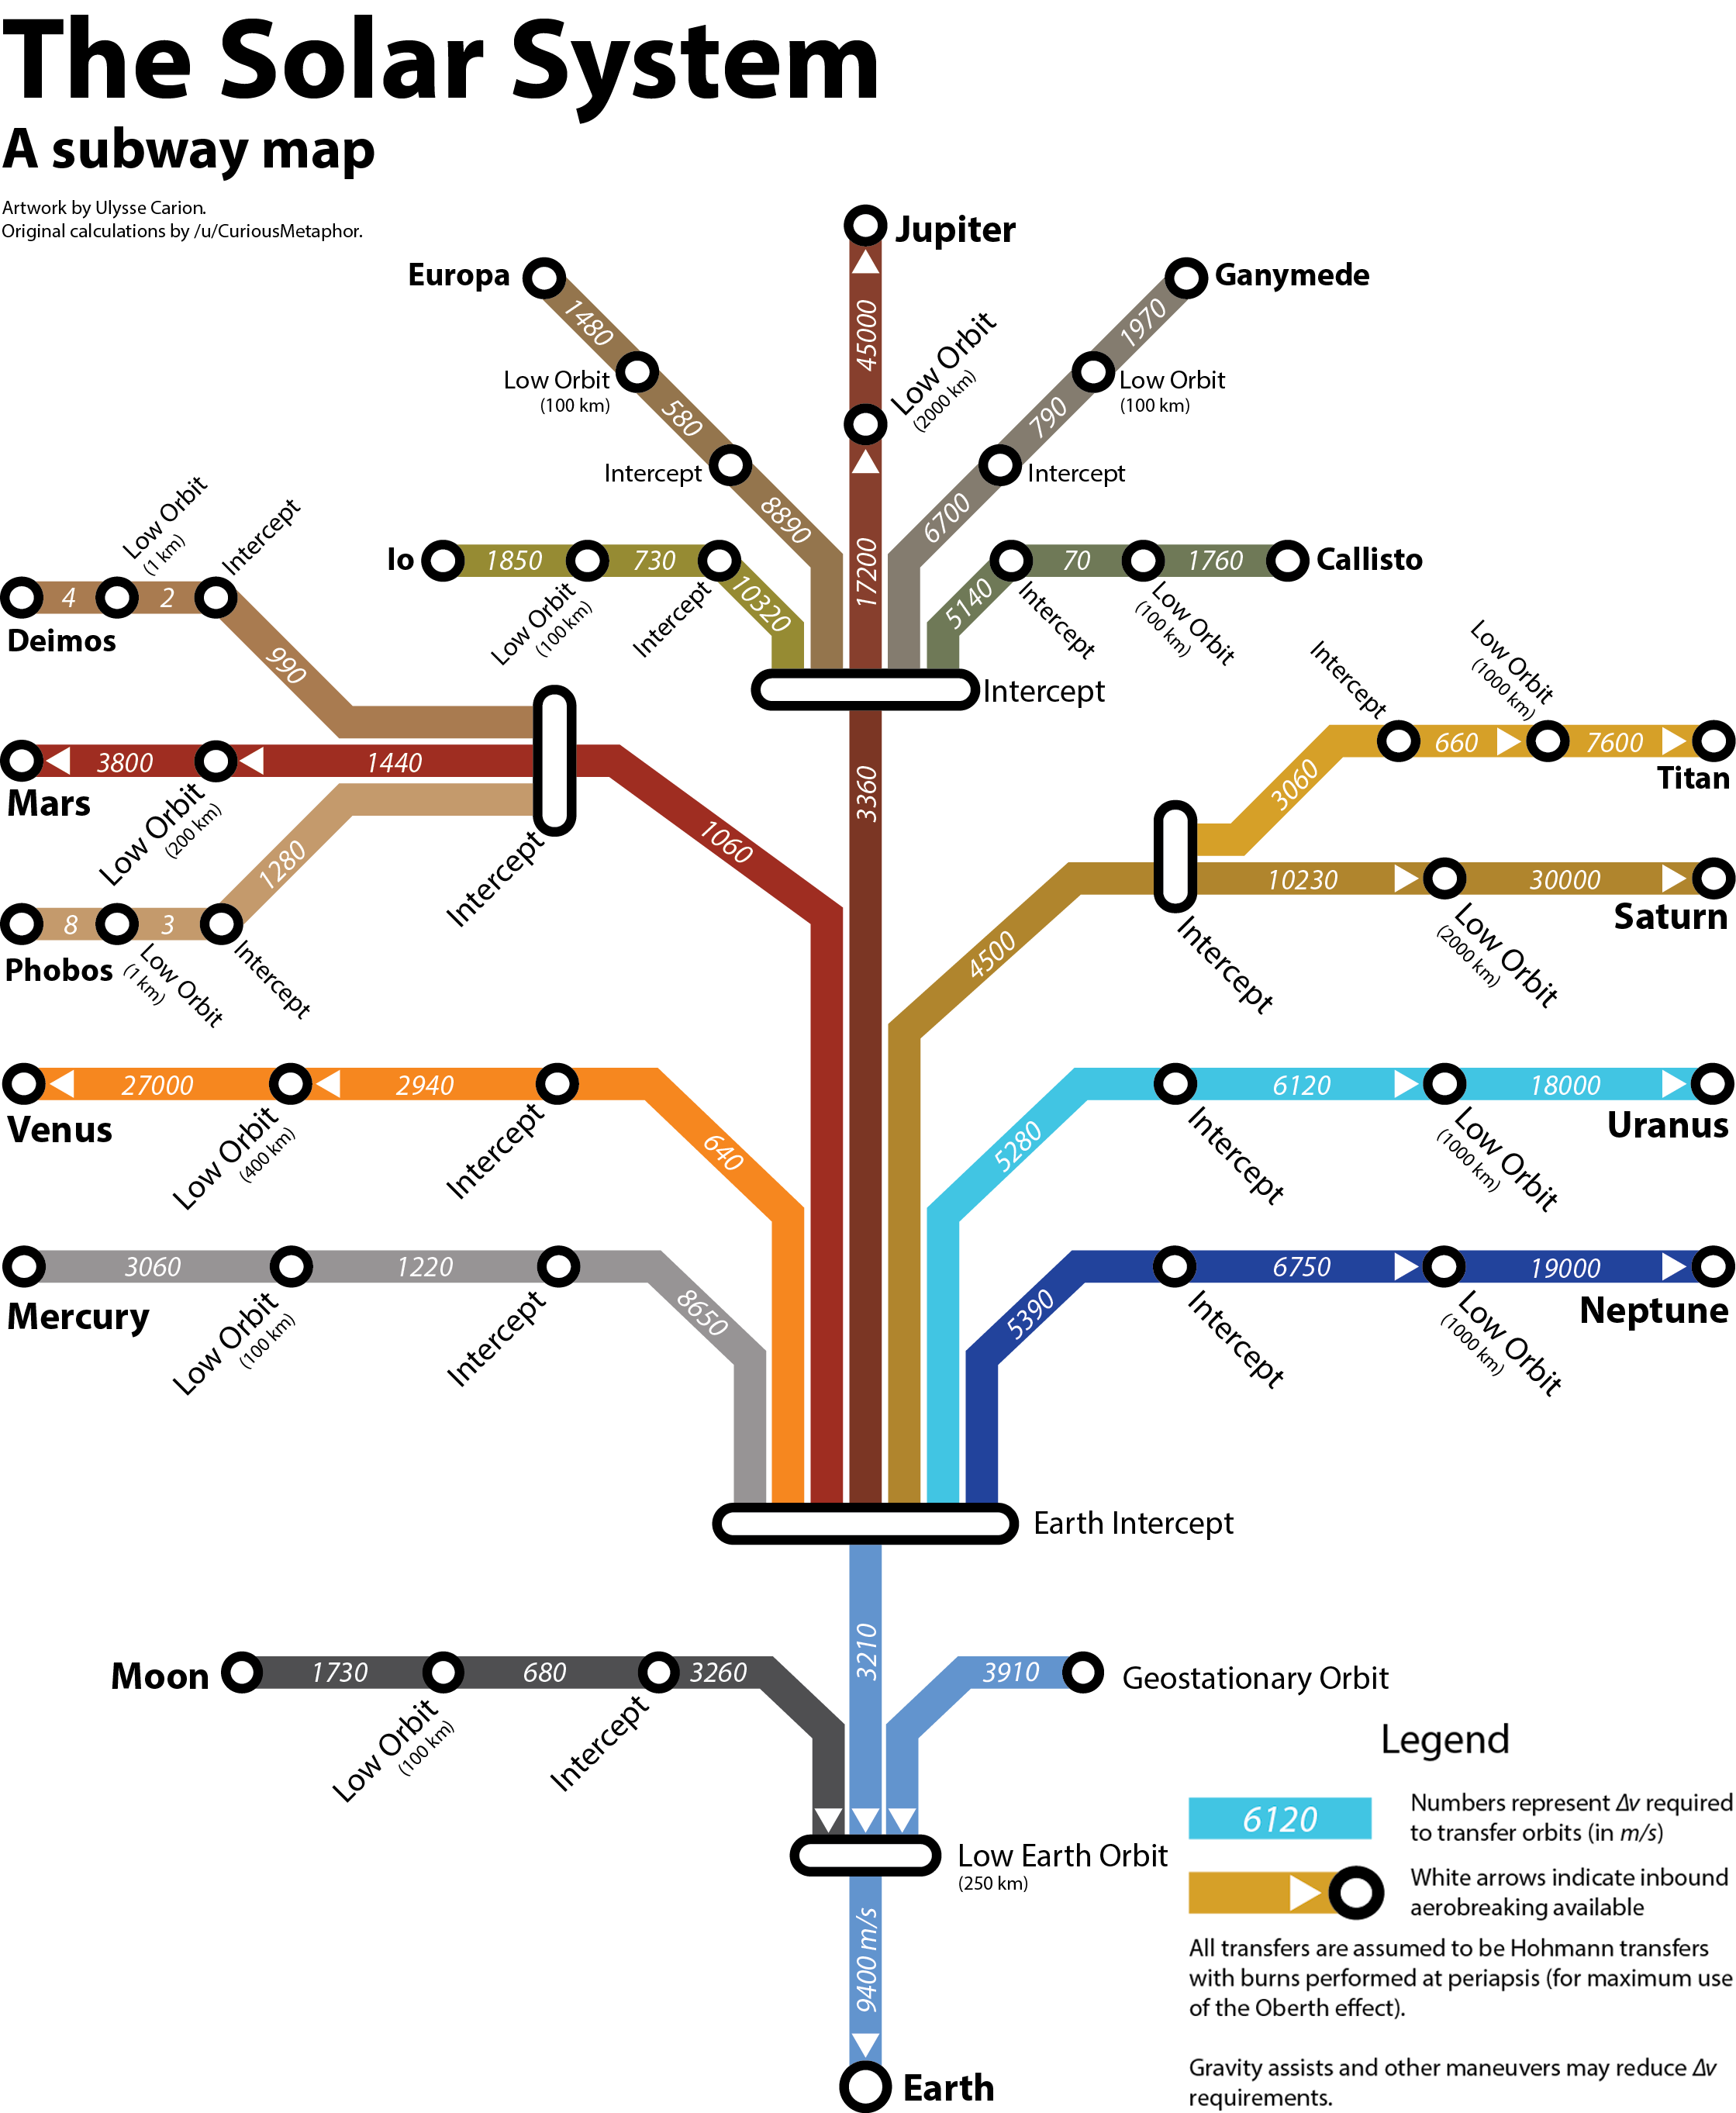
\includegraphics[width=\textwidth]{subway_map_legend}
  \caption{Representation of the different $\Delta V$ needed to go around the solar system, from \citet{reddit-subway}}
  \label{fig-subway_DV}
\end{figure}

\subsection{Rocket equation}
The thrust $T$ generated by ejecting mass at high velocity is
\begin{equation} \label{eq-thurst}
  T = v_{\rm ex} \dot{M}
\end{equation}
with $v_{\rm ex}$ the exhaust velocity of the propellant, and $\dot{M}$ the propellant mass flow rate through the thruster.
Hence,
\begin{equation} \label{eq-rocket}
  \Delta V = \int_{t_1}^{t_2} v_{\rm ex} \frac{ \norm{\dot{M}}}{M(t)} dt = v_{\rm ex} \ln \lp \frac{M_0}{M_1} \rp
\end{equation}
with $M_0 = M(t_0)$ and $M_1=M(t_1)$, and supposing that $v_{\rm ex}$ is constant.
We see from \cref{eq-rocket} that for a spacecraft of dry mass $M_1$ to have a given $\Delta V$, the exhaust velocity is directly linked to the initial \emph{wet} mass $M_0 = M_1 + M_{\rm prop}$, with $M_{\rm prop}$ the propellant mass.
\Cref{eq-rocket} is known as the (Tsiolkovsky) rocket equation.
Usually, instead of the exhaust velocity $v_{\rm ex}$, the specific impulse ${\Isp} = g_0 v_{\rm ex}$, with $g_0$ the standard gravity, is used.
\nomenclature[Q]{\ensuremath{ \Isp}}{ Specific impulse, related to the exhaust velocity of a propellant}
\nomenclature[P]{\ensuremath{ g_0}}{  Standard acceleration due to gravity \nomunit{9.80665 m/s$^2$}}

\subsection{Chemical space propulsion systems}
The usual rocket thruster uses a chemical reaction to generate the thrust.
For instance, the Vulcain (the thruster engine of the main stage of the European Ariane 5 and 6, developed by ArianeGroup, ex. Safran) uses the oxygen-hydrogen combustion, the most efficient chemical reaction \citep{nasa-H2O2}
\begin{equation*}
  2 {\rm H_2} + { \rm O_2} = 2 {\rm H_2 O} + 572 \text{~kJ},
\end{equation*}
with the energy of $572\,\kilo\joule$ of heat generated by $1\,\mole$ of oxygen.
This means that burning $1\,\kilo\gram$ of hydrogen-oxygen mixture generates a total energy of $13\,\mega\joule$. 
Supposing that the entire energy is converted into the exhaust of the water produced, its velocity would be of $5.1 \,\kms$.
In reality, the exhaust velocity of the Vulcain is of $4.2 \,\kms$, corresponding to $\Isp=431 \,\second$.
The efficiency of the Vulcain is close to 80\%, which is a very high efficiency, and it would be difficult to increase it significantly. 

In chemical propulsion systems, the fact that the energy released is related to the propellant mass gives an upper limit of exhaust velocity for a given combustion.
Electric propulsion engines, on the other hand, decouple the mass ejected (the propellant) from the energy source.
This decoupling allows a theoretical unlimited exhaust velocity.
Another advantage is the absence of reactive species, which lowers the security requirements impacting the spacecrafts.
Unfortunately, electric propulsion engines only work in vacuum and do not deliver sufficient thrust to compensate the earth gravity.
Hence, while electric propulsion can be used on spacecrafts, chemical propulsion is the only solution for rockets.

\subsection{Electric propulsion} \label{subsec-EP}
\ac{EP} systems mostly rely on plasmas \citep{charles2009,mazouffre2016}.
They have been successfully used since the 1960s by governments, but their complexity, the limited electric power available, and the inherent risk aversion of the space industry kept the \ac{EP} technologies hidden from the commercial applications \citep{lev2019}.
The breakthrough came in the '90s when the former Soviet Union's companies licensed the technology to western propulsion companies.
However, many commercial satellite manufacturers were skeptical, until the first decade of the 20th century, which brought strong evidence of the competitiveness of \ac{EP}.
The landmark of commercial use of \ac{EP} is the selling of four all-electric satellites for \ac{GEO} by Boeing in 2012, the first two of which were launched in March 2015.

The two leading \ac{EP} technologies used are
\begin{itemize}
  \item the \ac{HET}, also known as Stationary Plasma Thruster (SPT) in Russia
  \item the Gridded Ion Thruster (GIT), usually referred simply as Ion Thruster
\end{itemize}




 
 \paragraph{The Gridded Ion Thruster} is a plasma chamber closed at one end by two or more grids.
 The plasma source can be an emitting cathode, generating energetic electrons that ionize the propellant (usually Xenon), or a \ac{RF} source.
 The potential difference between the grids accelerates the ions.
 Another cathode is used to neutralize the ion beam.
 Compared to \ac{HET}s, it produces an ion beam with less divergence and a higher \Isp of the order of 3000 to 4000~s.
 \Cref{fig-iongridded} shows a picture of the ion thruster used for the BepiColombo mission toward Mercury.
 We see the neutralizing cathode, the accelerating grid, and the ion beam.
 
\begin{figure}[!hbt]
  \centering
  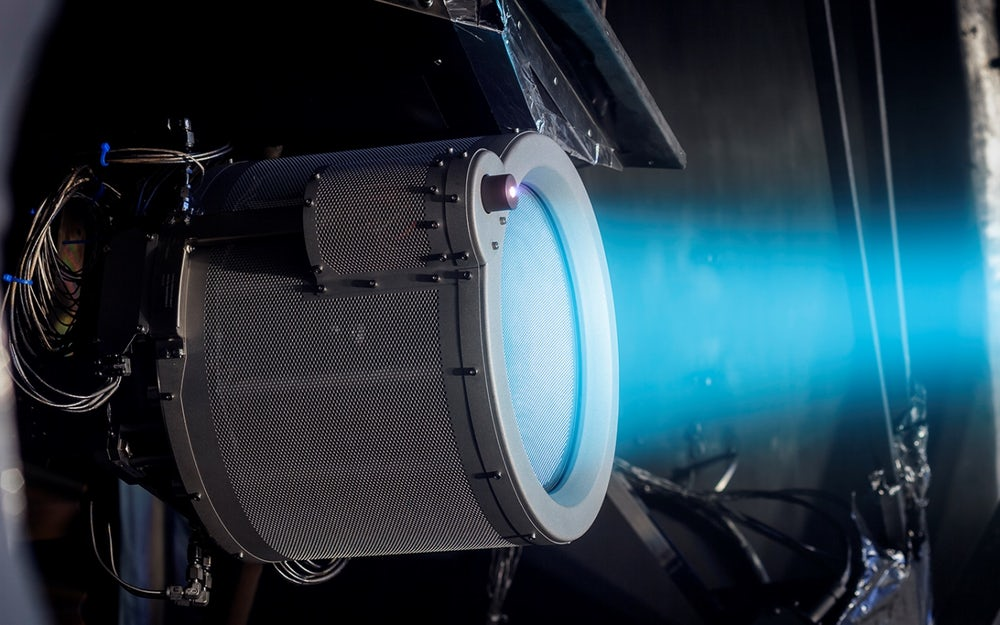
\includegraphics[width=\defaultwidth]{ion_Bepi}
  \caption{The T6 ion thruster will help send BepiColombo to Mercury. The neutralizing cathode is in the upper left quadrant of the thruster. (Credit\string: QinetiQ)}
  \label{fig-iongridded}
\end{figure}
 
 \paragraph{Hall Effect thrusters} use a magnetic barrier to both increase the ionization of the propellant and create the accelerating electric field.
 A detailed description of the \ac{HET} is presented in the next section.
 One cathode is used to start the discharge and neutralize the ion beam.
 Compared to GITs, \ac{HET}s need less power, hence reaching better thrust per power ratio and a smaller (therefore lighter) Power Processing Unit.
 Recently, the first satellites of two mega-constellations (OneWeb, 648 satellites planned, from which six were launched on February, the \nth{26} 2019, and Starlink, 12~000 satellites planned, from which 62 were launched on May, the \nth{23} 2019) were sent to Low Earth orbit, both using \ac{HET}s. 
 % Compared to GITs, \ac{HET}s need less power, and fewer power sources, hence reaching better thrust per power ratio and smaller (therefore lighter) Power Processing Unit. 
 Their typical \Isp is of the order of 1500~s.
 \Cref{fig-13kWHET} shows a high power prototype firing.
 We see the emitting cathode, in this design at the center, and the ion beam.
 \begin{figure}[!hbt]
   \centering
   \includegraphics[width=\defaultwidth]{HET_x3}
   \caption{A 13 kilowatt \acs{HET} prototype on a testing bench in a vacuum chamber (Credit\string: NASA).  }
   \label{fig-13kWHET}
 \end{figure}
 
 
 \subsection{EP environment in France} \label{subsec-HET_thruster}
 
 France is a leader country in the aerospace industry in both Europe and the world, with companies such as  Airbus, Thales, Safran, and ArianeGroup (join-venture of Safran and Airbus).
 As a consequence, the French ecosystem of electric propulsion is vibrant.
 The main thrusters produced in France are the PPS series by Safran, with the \PPS1350 (version G at 1.5~kW nominal power, and the version E at 2.7~kW), and the \PPS5000, a high power \ac{HET} at 5~kW, the first models of which have been delivered to Boeing in May 2019.
 A low-power version of the \PPS{}  is currently developed for low power, between 500\,W and 1\,kW\citep{vaudolon2018}.
 A list for the \PPS{} series elements and their respective characteristics can be seen in \cref{tab-ppsfamily}.
 \begin{table}[!hbt]
 \ra{1.3}
   \centering
   \caption{Members of the \PPS{} series developed by Safran Aircraft Engines \citep{boniface2017,duchemin2017,vaudolon2018}. The nominal operating condition of the \PPS{X00} is not fixed, yet.}
   \label{tab-ppsfamily}
   \begin{tabular}{@{}llll@{}} \toprule
   Name & Power & Thrust & \Isp \\ \midrule
   \PPS1350-G & 1.5~kW & 89~mN  & 1650~s \\
   \PPS1350-E & 2.7~kW & 140~mN  & 1800~s \\
   \PPS5000 & $3-5$~kW & $150-300$~mN  & $1850-1700$~s \\
   \PPS{X00} & $\sim 650$W &  $\sim$40~mN & $\sim 1450$~s \\
   \bottomrule
   \end{tabular}
 \end{table}
 
 Several initiatives concerning the small-sat sector are also undertaken, such as the start-ups Exotrail (micro \ac{HET}) and Thrust Me (radio frequency Ion Thruster), or the Electron Cyclotron Resonance Thruster at ONERA.
 Since 1996, numerous research projects have been carried out in France on HET with  the \ac{CNES}, SAFRAN and several research laboratories: ICARE, LAPLACE, CPHT, LPP, etc. \citep{boniface2017}.
 These numerous actors, combined with the support of the French and European space agencies, compose a stimulating environment that contributes both to the most mature technologies and the promising \ac{EP} concepts that could disrupt the propulsion sector.
 
% !TEX root=/home/tavant/these/manuscript/src/manuscript.tex

\section{Electric propulsion challenges}
\label{sec-challenges}
% \addcontentsline{toc}{section}{EP Industrial challenges}

Several challenges are currently tackled in the \ac{EP} industry.
The most prominent are listed by \citet{samukawa2012}\string:
\begin{enumerate}
  \item Performance improvement\string: efficiency, lifetime, and cost-effectiveness.
   Lifetime is an important issue and is limited by electrode or wall erosion.
   The lifetime of an electric thruster must be larger than 10 000 h of (reliable) operation.
   \item  Design of more versatile thrusters, i.e. able to operate at different combinations of thrust and propellant velocity.
   \item  Extension of the domain of operation to lower power ($\mu$N to 10 mN thrust range) for microsatellites or accurate attitude control.
   \item  Extension to higher power for orbit raising of telecommunication satellites (several tens of kW) and    interplanetary missions (100 kW and more).
   \item Extension of EP to low-altitude spacecraft\string: there is an increasing interest in civilian and military satellites flying  at altitudes around 100 km where the drag is significant and must be continuously compensated.
\end{enumerate}

\ac{HET} technology has the potential to answer many of these challenges.
For instance, the lifetime issue can be addressed with wall-less and magnetically shielded configurations.
Versatility is tackled with dual-mode \ac{HET} configuration \citep{boniface2017}, low power thruster is attained with $\mu$-thrusters \citep{lascombes2018}, and so forth.
However, the development of \ac{HET}s is slow and expensive. 
A better physical understanding of the processes governing \ac{HET}s is needed in order to reduce the cost and development times.
This is the objective of the current collaboration between Safran Aircraft Engines and \ac{LPP}.

% !TEX root=/home/tavant/these/manuscript/src/manuscript.tex


\section*{\acs{HET} research and development}
\label{sec-poseidon}
\addcontentsline{toc}{section}{\acs{HET} research and development}

Safran Aircraft Engines has been collaborating with \ac{LPP} since 2014, starting with the Ph.D. thesis of Viven Croes \citep{croes2017}.
During these first three years, a \ac{2D} \ac{PIC} code has been developed simulating the radial and azimuthal directions of a \ac{HET}.
Azimuthal instabilities have been observed in \citet{croes2017a}, and the effects of alternative propellants have been investigated in \citet{croes2018}.

From this fruitful collaboration, an ANR (Agence National de la Recherche) industrial chair {\sc Poseidon} for  "future Plasma thrusters for LOw earth orbit SatEllIte propulsiON systems", Grant No. ANR-16-CHIN-0003-01, has been created.
Its objective is to develop novel methods to reduce the development time and cost of the next \ac{EP} systems.
Both experiments and simulations are being developed to unlock the barriers of \ac{HET} development.
The {\sc Poseidon} chair is linked to the current development of a  low power \ac{HET} at Safran, the \PPS X00, which nominal operating point is of the order of 600W.
The scientific part of the chair is led by \ac{LPP}, while an unstructured \ac{3D} simulation code is developed by the CERFACS, in Toulouse.
Safran leads the technical development and experimental investigation.

At the beginning of my thesis, I participated in the development of a \ac{ML} of the \PPS X00.
The objectives of the \PPS X00-\ac{ML}  is to represent the physics of the \PPS X00 while allowing parametric studies of the main parameters of a \ac{HET}, such as the geometry, the magnetic field topology, or the wall material.
The \PPS X00-\ac{ML} has successfully shown its usefulness, as the first tests allow to obtain state of the art performances \citep{vaudolon2018}.
My work at Safran showed us that the development of \ac{HET} is still currently driven by experiments because numerical tools are not yet predictive.
Simulations can be helpful to engineers to obtain some insights for the thruster behavior, but cannot be used with confidence for development.
On the other hand, experiments are costly and time-consuming.
They also are prone to delays in the conception schedule, and reduce innovation as designers take fewer risks.

The lack of numerical tools comes from some physical phenomena that need to be better understood, even though \ac{HET} have been studied and used for more than 40 years.
% Hence a \emph{trial and errors} method is currently used by manufacturers for the development of the \ac{HET}.
These critical phenomena are \citep{samukawa2012,adamovich2017}
\begin{itemize}
  \item the electron transport,
  \item the plasma-surface interaction,
  \item the wall erosion,
  \item the propellant nature.
\end{itemize}

\vspace{1em}
The propellant nature impacts principally two things\string: the ion mass and the ionization energy.
Because of its high mass and low ionization energy, xenon has been used since the beginning of \ac{HET}. 
However, it is very costly, as it is mostly extracted from air with cryogenic distillation.
The atmosphere is composed in average of $\sn{9}{-6}\%$ of xenon \citep{earthfacs}.
The cheaper, but less effective, propellant of choice is krypton, which has recently started to be used.
Iodine could also be interesting, as it can be stored at room temperature in a solid state.
The impact of the propellant mass and chemistry is not yet clear and slows down the use of alternative propellants on already designed systems.

\vspace{1em}
The objectives of my thesis in the context of the {\sc Poseidon} chair focuses on the two first points -- the plasma wall interaction and the electron mobility -- and how they can influence each-other.
I also studied the wall erosion, but this work is classified, and will not be disclosed in this manuscript.






% !TEX root=/home/tavant/these/manuscript/src/manuscript.tex


\section*{Presentation of the Hall effect Thruster }
  \label{sec-HET}
  \addcontentsline{toc}{section}{Presentation of the Hall effect Thruster}

  
  The \ac{HET} is an electrostatic electrical propulsion system accelerating ions by the mean of an imposed voltage difference.
  \Cref{fig-bhtonoff} shows a picture of an \ac{HET} switched on and off.
  We can see the plasma in the annular plasma chamber.


  \begin{figure}[hbt]
    \centering
    \includegraphics[width=\defaultwidth]{PPS-ON_OFF.jpg}
    \caption{Front view off an \ac{HET}, the BHT-1500 from Busek, USA}
    \label{fig-bhtonoff}
  \end{figure}

  We can summarize the composition of an \ac{HET} with four parts\string:
  \begin{enumerate}
    \item The annular chamber.
    \item The injecting anode
    \item The cathode
    \item The magnetic circuit
  \end{enumerate}

  \begin{figure}[hbt]
    \centering
    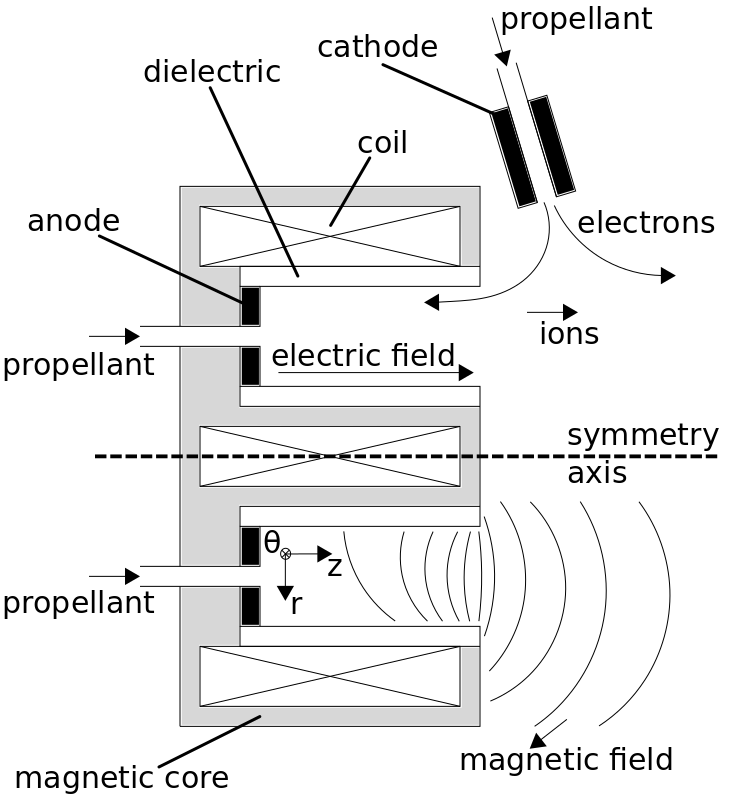
\includegraphics[width=\defaultwidth]{shematic_HET}
    \caption{Schematic cut of an \ac{HET}, illustrating its different parts. }
    \label{fig-shematiccut}
  \end{figure}

  \Cref{fig-shematiccut} presents a schematic cut of the \ac{HET} along its axial and radial direction.

  \paragraph{The chamber} has an annular shape.
  It is closed at the anode side and kept open at the other side.
  The axial length of the chamber is between $1$ and $3\,\centi\meter$; the radial width of the chamber is between $1$ and $2\,\centi\meter$. 
  The walls are usually constituted by a ceramic, as the \ac{BNSiO2}.
  The material needs to be resistant to erosion by ion impact sputtering.
  But changing the material is also known to affect the behavior of the discharge.
  The usually supposed phenomenon for this impact is the secondary electron emission yield that is a function of the material nature.
  For materials used in HET, this yield may be higher than one.


  \paragraph{The anode} is at the bottom of the chamber.
  The anode voltage is imposed to a few hundred volts.
  Usually, the neutral gas is injected through the anode itself, or close to the anode.
  The mass flow rate is of the order of a few mg/s.

  \paragraph{The cathode} is outside of the chamber.
  It is grounded, and injects electrons for two reasons\string:
  \begin{itemize}
    \item most of the electrons ($\sim 90 \%$) are used to neutralize the ion flux, for both allowing the ions to leave the thruster and avoiding charging of the spacecraft,
    \item  the others are attracted by the anode, hence entering the chamber. They enable the plasma discharge to switch and remain on.
  \end{itemize}

  \paragraph{The magnetic circuit} is composed of electromagnets and a magnetic circuit made of different ferromagnetic pieces.
  It creates a constant radial magnetic field in the annular chamber.
  The maximum value of the radial magnetic field is located close to the exit plane of the chamber.
  Its amplitude is on the order of $200$ Gauss ($\sn{2}{-2}$ T).

  \Cref{fig-bshape} illustrates the axial profile of the magnitude of the radial magnetic field.
  \begin{figure}[hbt]
    \centering
    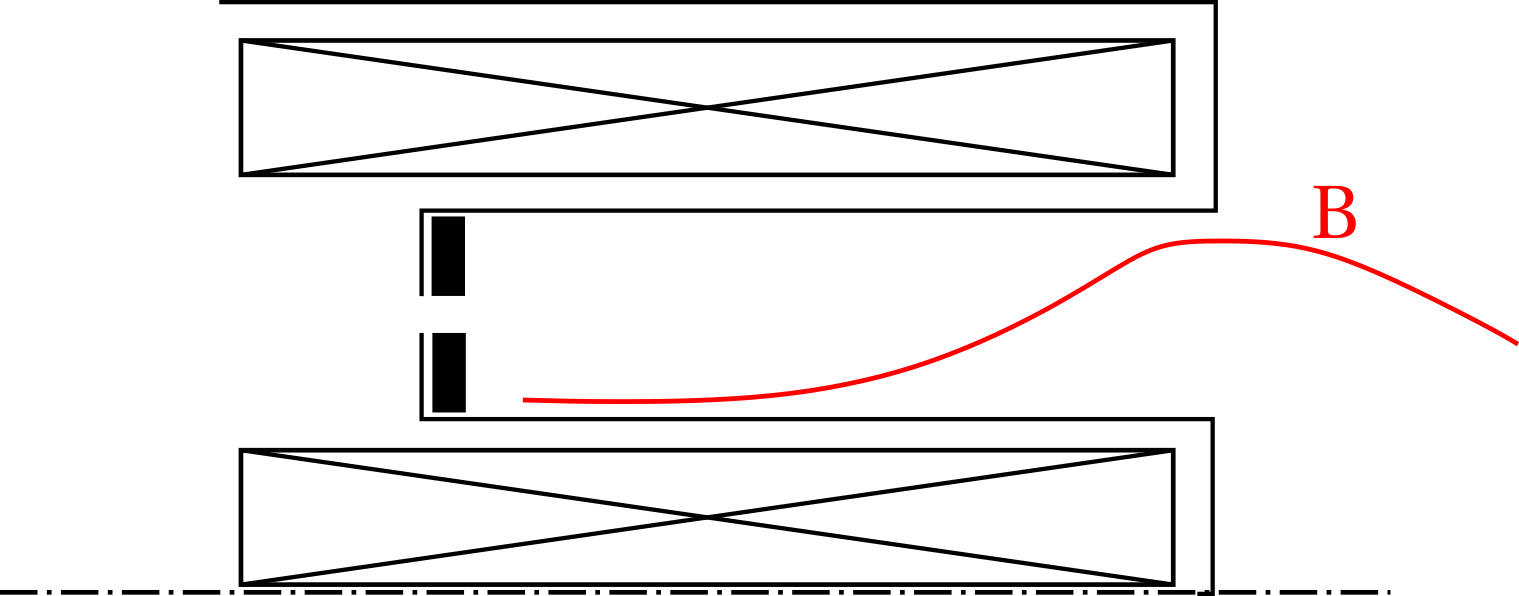
\includegraphics[width=\defaultwidth]{bshape}
    \caption{Usual shape of the axial profile of the radial magnetic field on the centerline of the channel.}
    \label{fig-bshape}
  \end{figure}


\section*{HET operating principle}
\addcontentsline{toc}{subsection}{HET operating principle}


  The operation principle of a \ac{HET} is rather simple.
  The objective is to ionize the propellant and impose an electric field to accelerate the ions.

  \paragraph{Ionization\\}
  The propellant, usually xenon, is ionized by electron-impact.
  The ionization energy needed is $\mathcal{E}_{\rm Xe, iz} = 12.13 \,\volt$, which corresponds to an electron velocity of $2000\,\kilo\meter\per\second$.
  Due to the low pressure (around $\sn{1}{-4}$ Pa), the mean free path of the electrons is larger than the chamber size.
  In consequence, a magnetic field is imposed in order to trap the electrons in a cyclotron motion.
  It increases the residence time of the electrons, thus promotes  ionization.
  In average in a well designed \ac{HET}, 90\% of the propellant is ionized.

  \paragraph{Acceleration\\}
  The potential difference  between the anode and the cathode is used to accelerate the ions outside of the chamber and create the thrust.
  Because the magnetic field slows the electrons down, the plasma resistivity increases in the region where the magnetic field amplitude is large.
  Hence, the axial profile of the magnitude of the axial electric field presents a maximum close to the maximum of the magnetic field.
  While the typical voltage difference is $U_d=300\,\volt$, the maximum electric field can be of the order of $30\,\kilo\volt\per\meter$ \citep{gawron2008}.

  \paragraph{Ionization and Acceleration regions overlap\\}
  \Cref{fig-zones} shows an illustration of the usual axial evolutions of the ionization and the electric and magnetic fields.
  As the magnetic field governs both the ionization and the acceleration regions, it can be challenging to obtain a clear separation between the two regions.
  However, if ionization happens in the acceleration region, the newly created ions will not be accelerated at their maximum velocity, hence resulting in a loss compared to the maximum theoretical thrust.
  The theoretical maximum speed is, by conservation of the total energy of the ion
  \begin{equation} \label{eq-vmaxtheo}
    v_{\rm ex, max} = \sqrt{ \frac{2 e V}{m_i} } \sim 31 \,\kilo\meter\per\second
  \end{equation}
  with $m_i = 131 \,\atomicmass$ for xenon and $V=300\,\volt$.


  \begin{figure}[hbt]
    \centering
    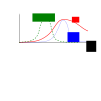
\includegraphics[width=\defaultwidth]{zones}
    \caption{Illustration of the usual axial profiles of the ionization and acceleration amplitude compared to the magnetic field.}
    \label{fig-zones}
  \end{figure}

  The thruster efficiency, in the usual configuration, is governed by its magnetic field topology.
  Hence, it can be tough to find the best topology that will optimize the ionization and the location of the ionization and acceleration regions.
  Some concepts of double stage \ac{HET} have been proposed to decouple the two phenomena to control them independently and are still under study \citep{dubois2018}.
  
  % However, the preliminary results are not as satisfactory as expected. 
  % \inlinenote{Add referecne here}
  % Moreover, the double-stage system needs more parts and power sources, resulting in a more complicated system.

  
  \section*{Instabilities present in the \ac{HET} }
  \label{sec-physics}
  \addcontentsline{toc}{subsection}{Instabilities present in the \ac{HET}}

  The \ac{HET}s are subject to numerous plasma oscillations, over a broad range of frequencies \citep{boeuf2017,choueiri2001}.
  The most important ones are\string:
  \begin{enumerate}
    \item Low frequency (10-20\,\kilo\hertz) ionization oscillations, usually referred to as breathing mode,
    \item Azimuthal low frequency rotating spokes, also in the \kilo\hertz{} range,
    \item Axial ion transit time oscillations, of the order of 100-500 \kilo\hertz,
    \item Azimuthal fast oscillations, of frequency of the order of the ion plasma frequency.
  \end{enumerate} 

  \paragraph{1. Breathing mode\\}
  The breathing mode is relatively well understood \citep{boeuf1998,barral2009,hara2014}.
  Indeed, a simple predator-prey model of two equations is enough to obtain the observed behaviour qualitatively.
  It is related to the idea that when the ionization is important, the neutral atom density decreases, reducing the ionization.
  Hence, the plasma density decreases, allowing the neutral density to rise again until the ionization grows up again.

  \paragraph{2. Rotating spokes\\}
  Experimental measurements with segmented anode \citep{ellison2012,mcdonald2011} seem to indicate that rotating spokes are present in the anode region.
  Their physical origins are less understood, as they were first attributed to ionization \citep{janes1966} but were later related to Simon-Hoh instability, and they were observed in \ac{PIC} simulations even with neglecting ionization \citep{carlsson2018}.
  However, in recent experiments, the presence of spokes did not seem to affect the \ac{HET} performances \citep{boeuf2018}.

  \paragraph{3. Transit time instability\\}
  Transit time instability has been predicted and observed in analytical and numerical models, respectively \citep{barral2005,boeuf2018}.
  Experimental studies of these instabilities are rather scarce, and it is only recently that time-resolved Laser-Induced Fluorescence measurements of the local ion velocity distribution function have confirmed the presence of this instability in a Hall thruster \citep{vaudolon2015}.
  This oscillation could reduce the performance of the thruster by increasing the overlap between the acceleration and ionization regions \citep{boeuf2018}.

  \paragraph{4. High-frequency azimuthal oscillations\\}
  These oscillations were first observed in \ac{PIC} simulations \citep{adam2004,ducrocq2006,adam2008a,heron2013} before being witnessed by electron Thomson scattering \citep{tsikata2009a,tsikata2009,tsikata2013}.
  They are essential, as they enhance the electron transport in the axial direction \citep{adam2004,lafleur2016a}.
  They are further described in the next section.

% !TEX root=/home/tavant/these/manuscript/src/manuscript.tex

\section*{Scientific challenges of the HETs}
\addcontentsline{toc}{section}{Scientific challenges of the HETs}

The scientific challenges are the critical phenomena not understood enough that prevent the industrial development of \ac{HET}s.
As introduced before, they concern the electron transport and the plasma-wall interaction.

\subsection*{Cross-field transport of the elections}
\addcontentsline{toc}{subsection}{Cross-field transport of the elections}

  \label{sec-mob}
  As a first approximation, the electrons are usually supposed frozen by the magnetic field.
  But in fact, they present a so-called cross-field transport toward the anode.
  For instance, because of collisions, the electrons can move from one magnetic line to another.
  This leads to a transport in the direction of the electric field.
  
  This transport can be expressed considering the electron momentum conservation equation \citep{lafleur2016a}\string:
  \begin{equation} \label{eq-elec_momentum_mobility}
    \partial_t(m_e n_e \vect{v}_{de}) + \grad \cdot (m_e n_e  \vect{v}_{de} \vect{v}_{de}) = q_e n_e ( \vect{E} + \vect{v}_{de} \times \vect{B}) - \grad \cdot \vect{\Pi}_e - m_e \nu_m n_e \vect{v}_{de},
  \end{equation}
  where $m_e, q_e$, $n_e$, $\vect{v}_{de}$, and $\vect{\Pi}_e $ are the electron mass, charge, density, drift velocity and pressure tensor, and $\nu_m$ is the electron-neutral momentum transfer collision frequency.
  Ignoring the electron inertia and the pressure term, and with $\vect{B} = B_0 \vect{e}_r$, we can write the conservation equation projected on the axial and azimuthal direction
  \begin{equation} \label{eq-elec_momentum_mobility2}
  \begin{cases}
    0 =  n_e E_z - n_e v_{de{\theta}} B_0 - \frac{m_e}{q_e} \nu_m n_e v_{dez}\\
    0 =  n_e E_{\theta} -  n_e v_{dez} B_0 - \frac{m_e}{q_e} \nu_m n_e v_{de{\theta}}
  \end{cases}
  \end{equation}
  Supposing that there is no electric field in the azimuthal direction ($E_{\theta}=0$),  we can combine the two equations of \cref{eq-elec_momentum_mobility2} and have \citep{chen2006,meezan2001}
  \begin{equation} \label{eq-mobility}
    \mobcla = \frac{n_e v_{dez}}{n_e E_z} = \frac{ \frac{\norm{q}}{m \nu_m}}{1 + \frac{\oce^2}{\nu_m}}
  \end{equation}
  with $\oce= \frac{\norm{q}B_0}{m}$ the cyclotron frequency.
  
  
  However, it has been observed in experiments by \citet{meezan2001} that the electron cross-field transport in the axial direction of the \ac{HET} is higher than $\mobcla$.
  Different phenomena have been proposed to explain the origin of this \emph{anomalous} transport.
  Two phenomena are supposed to be mainly responsible for this enhanced mobility \citep{croes2017}\string: the azimuthal instability and the near-wall mobility due to electron emission.
  A significant part of the work of this Ph.D. thesis concerns the quantitative comparison of the relative importance of the two phenomena.

  
  \subsection*{Electron drift and azimuthal instability in the HETs}
  \addcontentsline{toc}{subsection}{Electron drift and azimuthal instability in the HETs}

  The axial electric field $E$ and the radial magnetic field $B$ induces an azimuthal $E\times B$ drift of the electrons.
  The drift velocity $v_{\rm d, ExB}$ is 
  \begin{equation} \label{eq-exbdrift}
    v_{\rm d, ExB} = \bigg\lvert \frac{\vect{E} \times \vect{B}}{B^2} \bigg\rvert = \frac{E}{B} \sim \sn{1.5}{6} \,\meter\per\second
  \end{equation}
  Because of their large mass, the ions are not significantly affected by the magnetic field.
  Hence they do not drift azimuthally.
  As a consequence, there is a significant difference between the movement of electrons and ions in the azimuthal direction.

  This drift of electrons relative to the ions leads to instability in the azimuthal directions.
  Because the drift is perpendicular to the magnetic field, it is usually referred to as \ac{ECDI}.
  However, as it rises from an $E\times B$ drift, some authors use the name \ac{EDI}.
  In this thesis, we will use the name \ac{ECDI}.

  The actual nature of the \ac{ECDI} remains unclear\citep{boeuf2018}, as the \ac{ECDI} characteristics are very close to usual \ac{IAW}, and that experimental measurements are challenging to conduct in the range of parameter of interest.
  Hence, the community is still arguing about the actual nature of wave observed.
  A part of the work undertaken during my theses concerns the study and characterization of the instabilities observed in the kinetic simulations.
  These instabilities are treated in \cref{ch-5}.
  
\subsection*{Plasma-wall interaction}
\addcontentsline{toc}{subsection}{Plasma-wall interaction}

  The ceramic wall closes the chamber in the radial directions.
  It has been observed in experiments that the nature of the wall can significantly affect the discharge behavior \citep{gascon2003}.
  The primary phenomenon hold responsible for this observation is the electron emission.
  As usually observed in bounded plasmas, a floating sheath forms between the plasma and the dielectric wall.
  The sheath confines the electrons in the plasma and accelerates the ions toward the walls.
  This allows to obtain a flux of electrons equals to the flux of ions, resulting in charge conservation in the plasma, and a neutral flux, or also named zero-net current, to the surfaces.
  
  Due to the relatively high electron energy, the impact of a primary electron can lead to the emission of secondary electrons \citep{barral2003a,villemant2018}.
  The probability of \ac{SEE} depends on the electron impact characteristics (energy, angle) but also of the material\string: some materials are more emitting than others \citep{gascon2003}.
  Ion induced electron emission is much less likely to happen as the ions have a small impact energy.
  In addition to the near-wall conductivity discuss previously, these secondary electrons are accelerated toward the plasma by the sheath.
  Thus they modify the plasma and the sheath properties.
  Their impact on the electron temperature also affects the ionization rate, which is directly linked to the thruster efficiency.
  
  
  \citet{raitses2005} have observed that the current models of plasma-wall interactions with secondary electron emission cannot reproduce the electron temperature measured experimentally.
  The kinetic phenomena have been proposed by \citet{sydorenko2007} to explain this discrepancy between the models and the experiments.
  This could explain the differences between the kinetic simulations results and the global models in \citet{croes2017}.   
    
  \vspace{1em}
  In addition to \ac{SEE}, the ion impact energy is large enough to erode the walls by sputtering.
  This erosion is sufficient to be the main limitation of the lifetime of the \ac{HET}s.
  While most aspects of the erosion are well understood, we observe the apparition of  patterns with a typical scale of the order of the millimeter on the eroded surfaces.
  The origin and the possible implications of these erosion striations remain open questions.
  

\subsection*{Three-dimensional physics of the HET}
\label{sec-3Dphi}
\addcontentsline{toc}{subsection}{Three-dimensional physics of the HET}

The physics governing the \ac{HET} are three dimensional\string:
\begin{itemize}
  \item The plasma is accelerated in the axial direction by the electric field, and it is observed experimentally that the axial profile of the magnetic field is responsible for the performance of the thruster.
  \item The chamber walls close the radial dimension. The walls are responsible for most of the plasma losses, both on the particle and energy balances.
  \item The electrons drift in the azimuthal direction, leading to strong instabilities that affect the axial transport.
\end{itemize}

Consequently, when modeling or simulating a \ac{HET}, if one of the direction is not included, a part of the physics will be missing\string:
\begin{itemize}
  \item No axial direction\string: the ionization or the acceleration, as well as the plasma transport, are missing,
  \item No radial direction\string: the wall losses and interactions are missing,
  \item No azimuthal direction\string: the instability is missing. Hence the electron cross-field transport is not well represented.
\end{itemize}

While \ac{3D}-simulations have recently been proposed, they use scaling laws to simulate the system in a reasonable amount of time\citep{taccogna2019a}.
For instance, a reduced geometry is used in \citet{taccogna2018}, or a reduced density is used in \citet{fubiani2018a}.
A \ac{3D} simulation at real scale is not yet accessible.
Hence, we need to be able to rely on \ac{1D} or \ac{2D} simulations.
Consequently, we have to take into account the missing physics or include a model of its effects on the system.

% !TEX root=/home/tavant/these/manuscript/src/manuscript.tex


\section*{Plasma models and simulations}
\label{sec-simulations}
\addcontentsline{toc}{section}{Plasma models and simulations}

Depending on the pressure, energy, and time scale, different models are more adapted to describe the plasma.
There are mainly two distinct models.
The first is the \emph{kinetic} description of the species of the plasma, via the Boltzmann equation.
The second uses a \emph{fluid} description of the species, by means of moments.
% 
% \begin{figure}[hbtp]
%   \centering
%   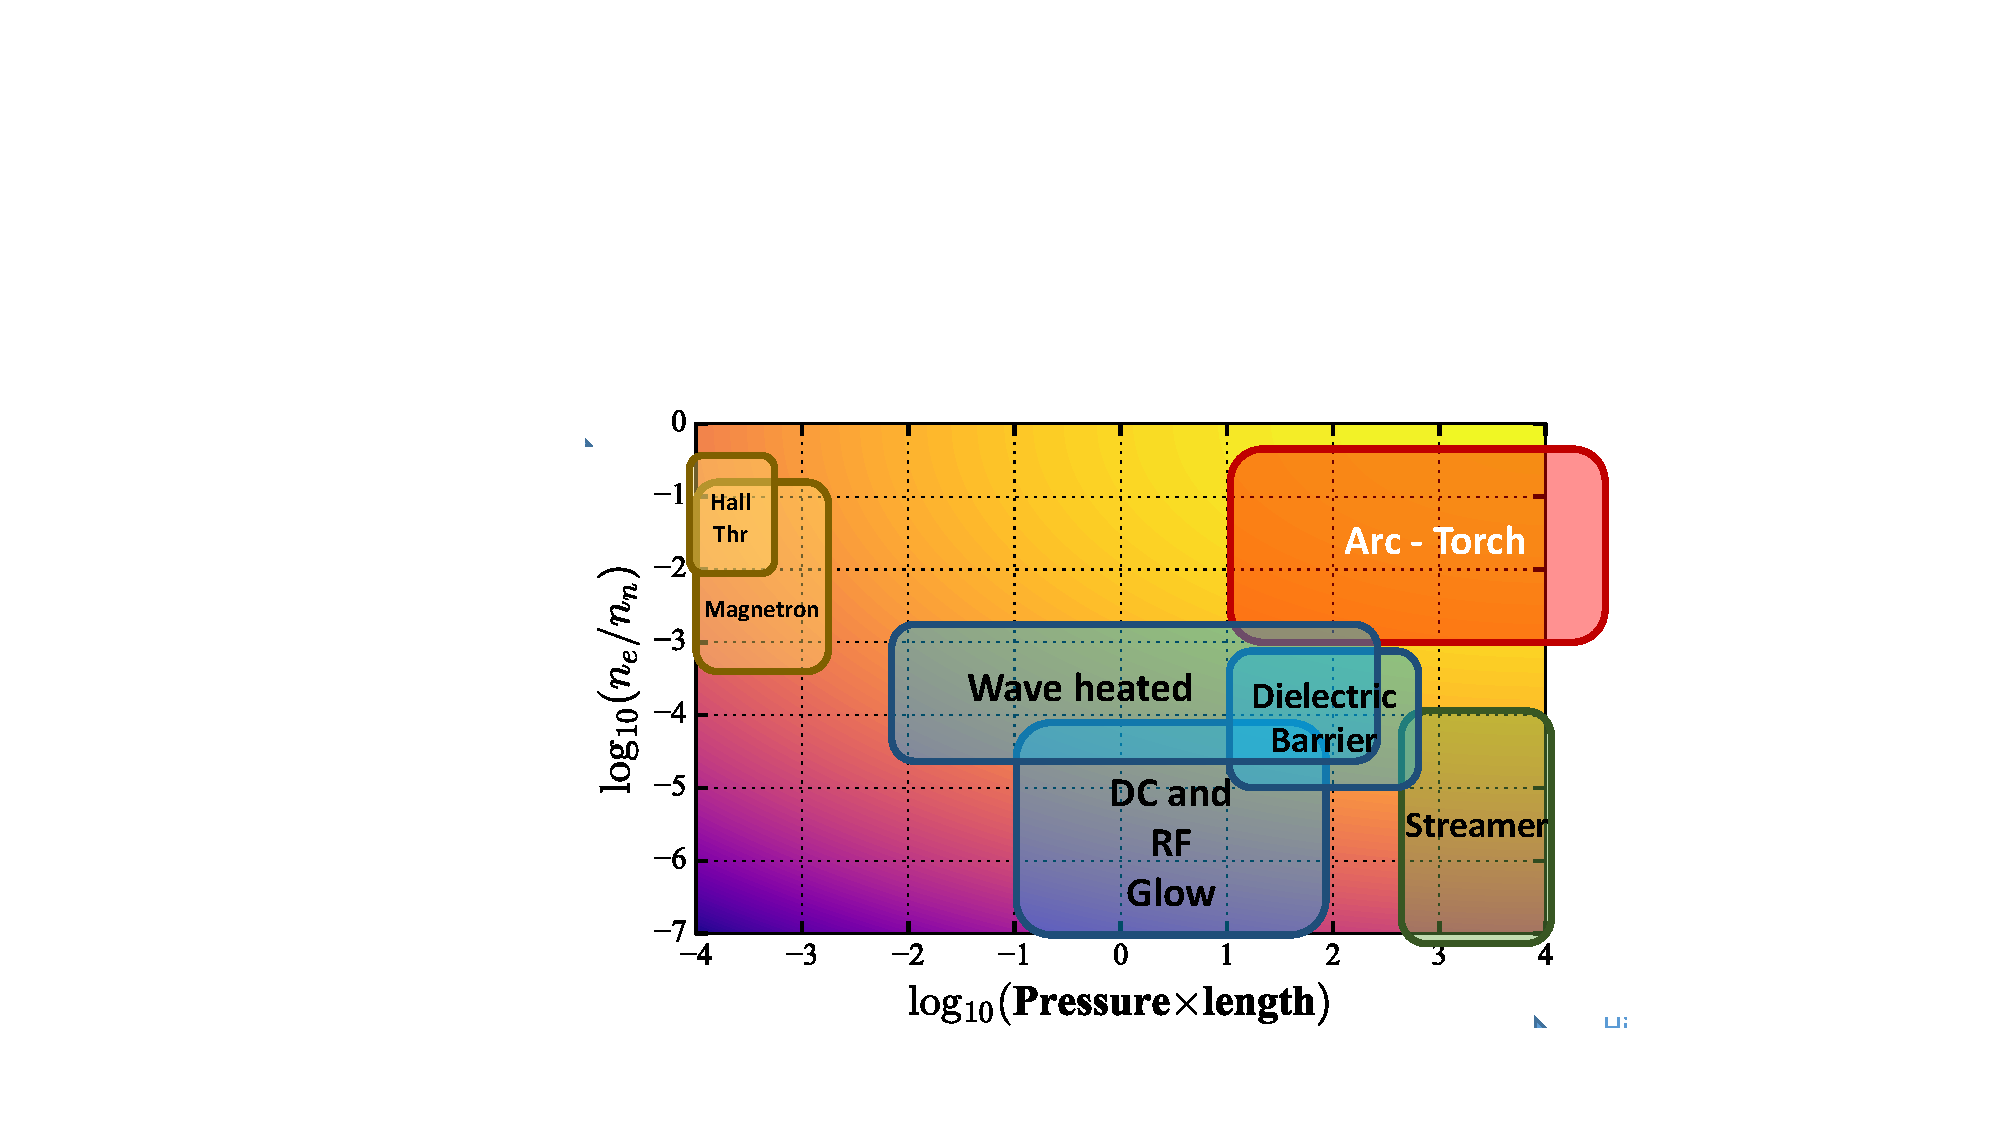
\includegraphics[width=\defaultwidth]{Chart}
%   \caption{}
%   \label{fig-chart}
% \end{figure}


\paragraph{Boltzmann equation \\}
The Boltzmann equation in \cref{eq-boltzmann} describes the evolution of the particles (atoms, ions and electrons) in the phase space.
The phase space is the set of each possible position $\vect{x}$ and velocity $\vect{v}$ that can be attained by a particle.
The evolutions in the phase space are due to forces, diffusion and collisions.

\begin{equation} \label{eq-boltzmann}
\deriv{f}{t}  + \vect{v} \cdot \grad_{\vect{x}} f + \vect{F} \cdot  \grad_{\vect{v}} f = \deriv{f}{t} \at{\rm coll}
\end{equation}
where $f$ is the distribution function of the particle at $\vect{x}, \vect{v}$, and $\deriv{f}{t}\mid_{\rm coll}$ denotes the effects of the collisions, $\grad$ is the gradient in both the positions (subscript $\vect{x}$) and the velocities (subscript $\vect{v}$)  and $\vect{F}$ is the force applied to the particle.
In the general electro-magnetic case,
\begin{equation*} \label{eq-forceEM}
  \vect{F} =  q \vect{E} + q \vect{v} \times \vect{B}
\end{equation*}
with $q$ the particle charge, $\vect{E}$ the electric field, and $\vect{B}$ the magnetic field.

\paragraph{Fluid equations \\}
The description on the plasma in 7 dimensions (3 of space, 3 of velocity, and one of time) can complicate the resolution of the Boltzmann equation.
If the precise description of $f$ is not needed, we can instead use the first moments of \Cref{eq-boltzmann} on the velocity in order to obtain a set of simpler equations.

The first equation is obtained by integrating \cref{eq-boltzmann} over the velocity space, which gives
\begin{align}
    & \iiint_{\vect{v}}  \deriv{f}{t} d^3v &&+&& \iiint_{\vect{v}}  \vect{v} \cdot \grad_{\vect{x}} f  d^3v &&+&&  \iiint_{\vect{v}}  \vect{F} \cdot  \grad_{\vect{v}} f  d^3v && = && \iiint_{\vect{v}}  \deriv{f}{t} \at{\rm coll} \nonumber  \\ 
   \iff &  \deriv{n}{t} &&+&&  \grad_{\vect{x}}  \cdot  ( \vect{u} n) &&+&& 0 &&=&& S_{\rm iz}   \label{eq-conc}
\end{align} 
where $n=\iiint f d^3v$ is the density, $\vect{u} = \frac{1}{n} \iiint \vect{v} f d^3v$ is the mean velocity, and $S_{\rm iz}$ is the source term of particle due to ionization.
\Cref{eq-conc} is the continuity equation for a given species.

In a similar fashion, integrating the Boltzmann equation times the velocity and the kinetic energy gives the momentum conservation equation and the energy conservation equation, respectively.
This set of equation is simpler to approach, although it relies on more hypotheses.

One of them is the closure of the system.
Indeed, the continuity equation describes the evolution of the density $n$ but needs the mean velocity $\vect{u}$.
However, the velocity is described by the momentum conservation equation that need the temperature $T$, and so on.
In order to close the system, one has to make a hypotheses on the higher moment of the distribution function.
A usual closure is the isothermal hypotheses, that fixes the temperature. 
Hence, the energy conservation equation is not needed.
Other closures possibles are the adiabatic hypotheses (no heath flux, the \nth{3} moment of $f$), the polytropic law linking the evolution of $n$ with $T$, or the Fourier law for heat diffusion.
% \inlinenote{Should we write the closes as equations ? $q = 0$, $T_e n_e ^{a}=cst$, etc. ?}


\subsection*{Plasma simulation models} \label{subsec-simulations}
As there are two different models to describe the plasma, there are two different simulation approaches \string: the fluid simulations and the kinetic simulations.
The fluid simulations solve the moments of the distribution function (the density, mean velocity and usually the temperature of the species), and the electromagnetic fields.
Depending of the conditions, the system of equation can be simplified before resolution.
In electrodynamic conditions, mainly for space plasmas and fusion, the Maxwell equations are coupled to the fluid equations leading to magnetohydrodynamics (MHD).
In the case of electrostatic conditions, as it is usual for Low Temperature plasmas, the Poisson equation is coupled to the fluid equations.
In most of low-temperature plasma, the plasma in quasi-neutral except in small regions as plasma sheaths close to walls.
It is also common to neglect inertia terms and assume a steady state in the momentum equations, leading to the drift-diffusion approximation
The fluid equations can be solved in \ac{3D}, \ac{2D} or \ac{1D} for space.
In low dimension model, the effects of the missing dimensions is usually added, for instance in the source terms as done by \citet{barral2003a}.


\vspace{1em}
However, some phenomena can only be described via the knowledge of the distribution function.
An example of such phenomena is the particle-wave interaction, as the Landau Damping \citep{landau1945,malmberg1964} or the plasma-beam instability \citep{filippychev1990}, for which the gradient of the distribution function in the velocity space is important.
In contrast to the fluid descriptions, \emph{kinetic} simulations solve the distribution function $f$ for both position and velocities.
Two approaches are usually used for kinetic simulations\string:
\begin{itemize}
  \item The \ac{DK} model, that discretize \Cref{eq-boltzmann} in the full phase space.
  \item The \ac{PIC} model, which uses an ensemble of particles to discretize the distribution function.
\end{itemize} 
While the \ac{DK} simulations use an Eulerian description of the distribution function, we can see the \ac{PIC} simulations as a Lagrangian approach.
The \ac{DK} simulations can theoretically better describe the plasma, mostly because there is less numerical noise and we can model binary collision more easily, especially Coulomb collisions.
On the other hand, \ac{PIC} simulations are much more simpler to develop on both a mathematical and a computation perspective.
For instance, the kinetic effect of electron emission have been recently studied using \ac{DK} simulation by \citet{cagas2019}, while it has been done since the last century in \ac{PIC} simulations \citep{boswell1988}.



% \input{Context/6_LPPic}
% !TEX root=/home/tavant/these/manuscript/src/manuscript.tex

\section{Problem statement and outline of the thesis}
\label{sec-problematic}
% \addcontentsline{toc}{section}{Problematic of the thesis}

My thesis takes part of the collaboration between Safran Aircraft Engines and the Laboratory of Plasma Physics, which objective is to study the fundamental physics governing the \ac{HET}, in the optic to accelerate the developments of the next generations of thrusters.
I mainly focused on the electron transport and the plasma-wall interaction,
both aspects requiring the use of kinetic tools.

Indeed, the electron transport is affected by instabilities that can only be described by kinetic models \citep{adam2008a,lafleur2016a}.
Furthermore, the plasma-wall interaction is also affected by kinetic effects, both concerning the electron emission induced by electron impact \citep{barral2003a,raitses2011,sydorenko2006} and the wall erosion by ion impact sputtering.
Relatively few simulation codes highly parallelized have been developed, that could allow parametric studies.
But the ever-increasing computational power available allows bigger simulations to be conducted.
Thus, a significant part of my work involves the development of a highly efficient \ac{PIC} simulation code, with all of the technical difficulties related to it.
The simulation code is then used to proceed to several parametric studies, that I used to derive reliable low-dimensional models that could be used to derive new engineering development tools.


\vspace{1em}
In \cref{ch-1}, we introduce \LPPic, the primary simulation model used in this work, with an emphasis on the axial convection of the particles and the plasma-wall interaction.
\cref{ch-5} focus on the azimuthal instability observed in the simulation and compares it to the dispersion relation.
\cref{ch-2} presents the results of a parametric study investigating the wall effect.
In \cref{ch-3,ch-4}, we modify the sheath model in order to reproduce the \ac{PIC} simulation results.
\cref{ch-3} focuses on a simplified \ac{1D} simulation to study the electron state law, while \cref{ch-4} continues the same model by including the secondary electron emission.
While the majority of the work studied the \ac{2D} radial and azimuthal simulation, we finish by study the radial direction in a \ac{2D} axial and azimuthal simulation in \cref{ch-6}.



% Remove the setting for the introduction
\let\leftmark=\oldleftmark
\let\rightmark=\oldrightmark

\renewcommand\thechapter\oldthechapter
\renewcommand\theHchapter\oldtheHchapter
\renewcommand\chaptername{Chapter}